\section{pbdR}
\makesubcontentsslides

\subsection{The pbdR Project}

\begin{frame}
  \begin{block}{\pbdR\ Packages}
    \begin{center}
      \begin{columns}\hspace{.2cm}
        \begin{column}{.52\textwidth}
          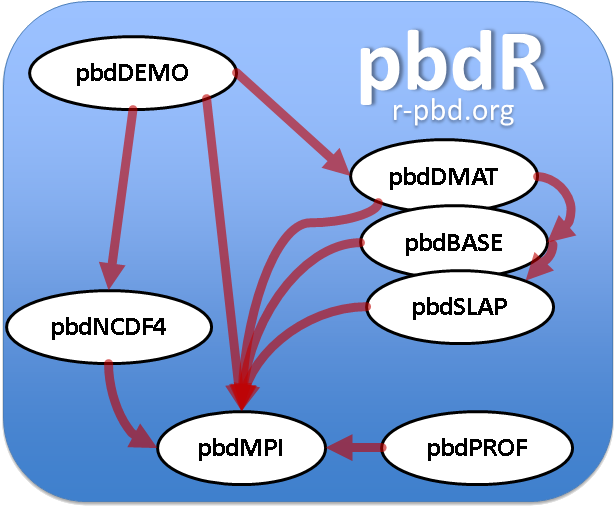
\includegraphics[scale=.4]{../common/pics/pbdR}
        \end{column}
        \hspace{.05cm}
        \begin{column}{.4\textwidth}
          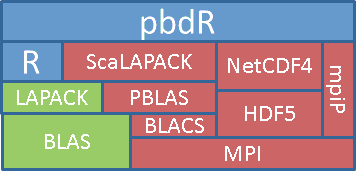
\includegraphics[scale=.45]{../common/pics/libs}
        \end{column}
      \end{columns}
    \end{center}
  \end{block}
\end{frame}

\subsection{pbdMPI}

\begin{frame}[fragile]
  \begin{block}{Simplified Interface for MPI Operations with \textbf{pbdMPI}}\pause
    \begin{minipage}[t]{.475\textwidth}
      \begin{lstlisting}[title=Rmpi]
# int
mpi.allreduce(x, type=1)
# double
mpi.allreduce(x, type=2)
     \end{lstlisting}
   \end{minipage}
   \hfill
   \begin{minipage}[t]{.475\textwidth}
     \begin{lstlisting}[title=pbdMPI]
allreduce(x)
     \end{lstlisting}
     \vspace{1em}
     \hspace{1em}{\small S4. Batch only! (No spawning)}
   \end{minipage}
 \end{block}
%
 \begin{block}{Types in R}
   \vspace{-.2cm}
   \begin{lstlisting}
> is.integer(1)
[1] FALSE
> is.integer(2)
[1] FALSE
> is.integer(1:2)
[1] TRUE
   \end{lstlisting}
 \end{block}
\end{frame}

\begin{frame}
  \begin{block}{MPI Operations: The Gang's All Here}\pause
    \begin{itemize}
      \item \textbf{Communicator wrangling}: {\color{blue}\code{init()},   
\code{finalize()}}\\[.4cm]
      %
      \item \textbf{Rank query}: {\color{blue}\code{comm.rank()}, \code{comm.size()}}\\[.4cm]
      %
      \item \textbf{Reduction}: \code{reduce(x, op='sum')},     
{\color{blue}\code{allreduce(x)}}\\[.4cm]
      %
      \item \textbf{Gather}: \code{gather(x)}, {\color{blue}\code{allgather(x)}}\\[.4cm]
      %
      \item \textbf{Broadcast}: \code{bcast(x)}\\[.4cm]
      %
      \item \textbf{Barrier}: \code{barrier()}\\[.4cm]
      %
      \item \textbf{Send/Receive}: \code{send(x)}, \code{recv()}
    \end{itemize}
  \end{block}
\end{frame}


\begin{frame}
  \begin{block}{MPI Operations for R Users}\pause
    \begin{itemize}
      \item \textbf{Printing}:  \code{comm.print(x)}, \code{comm.cat(x)}\\[.4cm]
      %
      \item \textbf{RNG Seeds}: \code{comm.set.seed(diff=T)}\\[.4cm]
      %
      \item \textbf{Task Subsetting}: \code{get.jid(n)}\\[.4cm]
      %
      \item \textbf{*ply}: \\
      \code{pbdApply(X, MARGIN, FUN, \dots)}\\
      \code{pbdLapply(X, FUN, \dots)}\\
      \code{pbdSapply(X, FUN, \dots)}\\
    \end{itemize}
  \end{block}
\end{frame}


\begin{frame}[fragile]
  \begin{exampleblock}{SPMD Rank Query Example}
  \centering
\begin{lstlisting}[title=1\_rank.r]
library(pbdMPI, quiet = TRUE)
init()

my.rank <- comm.rank()
comm.print(my.rank, all.rank=TRUE)

finalize()
\end{lstlisting}
  \begin{columns}[t,onlytextwidth]
    \begin{column}{0.62\textwidth}
\begin{lstlisting}[backgroundcolor=\color{white},keywordstyle=\color{black},
title=Execute this batch script via:]
mpirun -np 2 Rscript 1_rank.r
\end{lstlisting}    
    \end{column}
    \hfill
    \begin{column}{0.35\textwidth}
\begin{lstlisting}[title=Sample Output:]
COMM.RANK = 0
[1] 0
COMM.RANK = 1
[1] 1
\end{lstlisting}
    \end{column}
​  \end{columns}
  \end{exampleblock}
\end{frame}

\subsection{pbdDMAT}

\begin{frame}[shrink]
\begin{exampleblock}{2$\times$3 block-cyclic grid on 6 processors:
    Global view ``ddmatrix'' class}
\begin{align*}
x &= \left[
      \begin{array}{ll|ll|ll|ll|l}
      \color{g11}x_{11} & \color{g11}x_{12} & \color{g12}x_{13} & \color{g12}x_{14} & \color{g13}x_{15} & \color{g13}x_{16} & \color{g11}x_{17} & \color{g11}x_{18} & \color{g12}x_{19}\\
      \color{g11}x_{21} & \color{g11}x_{22} & \color{g12}x_{23} & \color{g12}x_{24} & \color{g13}x_{25} & \color{g13}x_{26} & \color{g11}x_{27} & \color{g11}x_{28} & \color{g12}x_{29}\\\hline
      \color{g21}x_{31} & \color{g21}x_{32} & \color{g22}x_{33} & \color{g22}x_{34} & \color{g23}x_{35} & \color{g23}x_{36} & \color{g21}x_{37} & \color{g21}x_{38} & \color{g22}x_{39}\\
      \color{g21}x_{41} & \color{g21}x_{42} & \color{g22}x_{43} & \color{g22}x_{44} & \color{g23}x_{45} & \color{g23}x_{46} & \color{g21}x_{47} & \color{g21}x_{48} & \color{g22}x_{49}\\\hline
      \color{g11}x_{51} & \color{g11}x_{52} & \color{g12}x_{53} & \color{g12}x_{54} & \color{g13}x_{55} & \color{g13}x_{56} & \color{g11}x_{57} & \color{g11}x_{58} & \color{g12}x_{59}\\
      \color{g11}x_{61} & \color{g11}x_{62} & \color{g12}x_{63} & \color{g12}x_{64} & \color{g13}x_{65} & \color{g13}x_{66} & \color{g11}x_{67} & \color{g11}x_{68} & \color{g12}x_{69}\\\hline
      \color{g21}x_{71} & \color{g21}x_{72} & \color{g22}x_{73} & \color{g22}x_{74} & \color{g23}x_{75} & \color{g23}x_{76} & \color{g21}x_{77} & \color{g21}x_{78} & \color{g22}x_{79}\\
      \color{g21}x_{81} & \color{g21}x_{82} & \color{g22}x_{83} & \color{g22}x_{84} & \color{g23}x_{85} & \color{g23}x_{86} & \color{g21}x_{87} & \color{g21}x_{88} & \color{g22}x_{89}\\\hline
      \color{g11}x_{91} & \color{g11}x_{92} & \color{g12}x_{93} & \color{g12}x_{94} & \color{g13}x_{95} & \color{g13}x_{96} & \color{g11}x_{97} & \color{g11}x_{98} & \color{g12}x_{99}\\
      \end{array}
\right]_{9\times 9}
\end{align*}
\begin{align*}
\text{Processor grid = }\left|
      \begin{array}{lll}
      \color{g11}0 & \color{g12}1 & \color{g13}2\\
      \color{g21}3 & \color{g22}4 & \color{g23}5
      \end{array}
\right| &= 
\left|
      \begin{tabular}{lll}
      \color{g11}(0,0) & \color{g12}(0,1) & \color{g13}(0,2)\\
      \color{g21}(1,0) & \color{g22}(1,1) & \color{g23}(1,2)
      \end{tabular}
\right|
\end{align*}
\end{exampleblock}
\end{frame}


\begin{frame}[shrink]
\begin{exampleblock}{2$\times$3 block-cyclic grid on 6 processors:
    Local view ``ddmatrix'' class}
\begin{align*}
\left[
      \begin{array}{ll|ll}
      \color{g11}x_{11} & \color{g11}x_{12} & \color{g11}x_{17} & \color{g11}x_{18}\\
      \color{g11}x_{21} & \color{g11}x_{22} & \color{g11}x_{27} & \color{g11}x_{28}\\\hline
      \color{g11}x_{51} & \color{g11}x_{52} & \color{g11}x_{57} & \color{g11}x_{58}\\
      \color{g11}x_{61} & \color{g11}x_{62} & \color{g11}x_{67} & \color{g11}x_{68}\\\hline
      \color{g11}x_{91} & \color{g11}x_{92} & \color{g11}x_{97} & \color{g11}x_{98}\\
      \end{array}
\right]_{5\times 4}
\left[
      \begin{array}{ll|l}
      \color{g12}x_{13} & \color{g12}x_{14} & \color{g12}x_{19}\\
      \color{g12}x_{23} & \color{g12}x_{24} & \color{g12}x_{29}\\\hline
      \color{g12}x_{53} & \color{g12}x_{54} & \color{g12}x_{59}\\
      \color{g12}x_{63} & \color{g12}x_{64} & \color{g12}x_{69}\\\hline
      \color{g12}x_{93} & \color{g12}x_{94} & \color{g12}x_{99}\\
      \end{array}
\right]_{5\times 3}
\left[
      \begin{array}{ll}
      \color{g13}x_{15} & \color{g13}x_{16}\\
      \color{g13}x_{25} & \color{g13}x_{26}\\\hline
      \color{g13}x_{55} & \color{g13}x_{56}\\
      \color{g13}x_{65} & \color{g13}x_{66}\\\hline
      \color{g13}x_{95} & \color{g13}x_{96}\\
      \end{array}
\right]_{5\times 2}
\\
\left[
      \begin{array}{ll|ll}
      \color{g21}x_{31} & \color{g21}x_{32} & \color{g21}x_{37} & \color{g21}x_{38}\\
      \color{g21}x_{41} & \color{g21}x_{42} & \color{g21}x_{47} & \color{g21}x_{48}\\\hline
      \color{g21}x_{71} & \color{g21}x_{72} & \color{g21}x_{77} & \color{g21}x_{78}\\
      \color{g21}x_{81} & \color{g21}x_{82} & \color{g21}x_{87} & \color{g21}x_{88}\\
      \end{array}
\right]_{4\times 4}
\left[
      \begin{array}{ll|l}
      \color{g22}x_{33} & \color{g22}x_{34} & \color{g22}x_{39}\\
      \color{g22}x_{43} & \color{g22}x_{44} & \color{g22}x_{49}\\\hline
      \color{g22}x_{73} & \color{g22}x_{74} & \color{g22}x_{79}\\
      \color{g22}x_{83} & \color{g22}x_{84} & \color{g22}x_{89}\\
      \end{array}
\right]_{4\times 3}
\left[
      \begin{array}{ll}
      \color{g23}x_{35} & \color{g23}x_{36} \\
      \color{g23}x_{45} & \color{g23}x_{46} \\\hline
      \color{g23}x_{75} & \color{g23}x_{76} \\
      \color{g23}x_{85} & \color{g23}x_{86} \\
      \end{array}
\right]_{4\times 2}
\end{align*}
\begin{align*}
\text{Processor grid = }\left|
      \begin{array}{lll}
      \color{g11}0 & \color{g12}1 & \color{g13}2\\
      \color{g21}3 & \color{g22}4 & \color{g23}5
      \end{array}
\right| &= 
\left|
      \begin{tabular}{lll}
      \color{g11}(0,0) & \color{g12}(0,1) & \color{g13}(0,2)\\
      \color{g21}(1,0) & \color{g22}(1,1) & \color{g23}(1,2)
      \end{tabular}
\right|
\end{align*}
\end{exampleblock}
\end{frame}

\begin{frame}[fragile]
  \begin{block}{\pbdR\ Example Syntax}
  \begin{lstlisting}
x <- x[-1, 2:5]
x <- log(abs(x) + 1)
x.pca <- prcomp(x)
xtx <- t(x) %*% x
ans <- svd(solve(xtx))
  \end{lstlisting}
  \begin{center}
  \emph{The above (and over 100 other functions) runs on 1 core with R \\
    or 10,000 cores with \pbdR ddmatrix class}
  \end{center}
\begin{lstlisting}
> showClass("ddmatrix")
Class "ddmatrix" [package "pbdDMAT"]

Slots:
                                              
Name:     Data     dim    ldim   bldim   ICTXT
Class:  matrix numeric numeric numeric numeric
\end{lstlisting}
  \end{block}
\end{frame}

\subsection{pbdPROF}

\begin{frame}[fragile]
  \begin{block}{Profiling with \textbf{pbdPROF}}
  \begin{minipage}[t]{.58\textwidth}
  \vspace{0pt}
  1. Rebuild \pbdR\ packages
\vspace*{-.5cm}
\begin{lstlisting}[language=shl,title=\ ]
R CMD INSTALL pbdMPI_0.2-1.tar.gz \ --configure-args= \ "--enable-pbdPROF"
\end{lstlisting}
2. Run code
\vspace*{-.5cm}
\begin{lstlisting}[language=shl,title=\ ]
mpirun -np 64 Rscript my_script.R
\end{lstlisting}

3. Analyze results
\vspace{-.5cm}
\begin{lstlisting}[title=\ ]
library(pbdPROF)
prof <- read.prof( "profiler_output.mpiP")
plot(prof)
\end{lstlisting}
  \end{minipage}
  \hfill
  \begin{minipage}[t]{.4\textwidth}
  \vspace{0pt}
    \centering
    Publication-quality graphs\\
    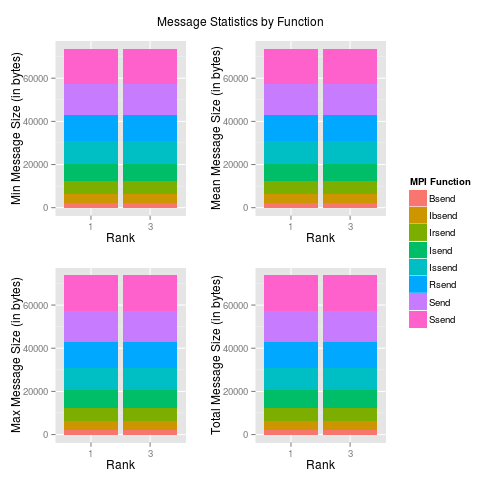
\includegraphics[scale=.25]{../common/pics/mpip}
    \\[.1cm]
    
\includegraphics[scale=0.3]{../common/pics/gsoc}
  \end{minipage}
  \centering
  Supports fpmpi and mpiP.  Expanding this fall to include support for TAU!
  \end{block}
\end{frame}

\subsection{pbdPAPI}

\begin{frame}[fragile]
  \small
  \begin{block}{pbdPAPI: Performance Application Programming Interface}
    \begin{minipage}[t]{.75\textwidth}
      \vspace{0pt}
      \begin{itemize}
      \item Cache miss/hit/read/write, flops, instructions, \dots
      \item Deeply profile \emph{any} R code.
      \item On Github: ``RBigData/pbdPAPI''
      \item See blog about pbdPAPI on R-bloggers.com
      \end{itemize}
    \end{minipage}
    \hfill
    \begin{minipage}[t]{.2\textwidth}
      \vspace{0pt}
      \hspace*{-.7cm}
      
\includegraphics[width=1.2\textwidth]{../common/pics/gsoc_2014}
    \end{minipage}
    \begin{lstlisting}
> library(pbdPAPI)
> system.cache(x <- rnorm(1e5), type="miss", events="l2.ratio")
L2 cache miss ratio 
          0.1080902 

> system.flops(x/100)[3:4]
$flpops
[1] 100237

$mflops
[1] 107.0419
    \end{lstlisting}
  \end{block}
\end{frame}

